% Options for packages loaded elsewhere
\PassOptionsToPackage{unicode}{hyperref}
\PassOptionsToPackage{hyphens}{url}
%
\documentclass[
  ignorenonframetext,
]{beamer}
\usepackage{pgfpages}
\setbeamertemplate{caption}[numbered]
\setbeamertemplate{caption label separator}{: }
\setbeamercolor{caption name}{fg=normal text.fg}
\beamertemplatenavigationsymbolsempty
% Prevent slide breaks in the middle of a paragraph
\widowpenalties 1 10000
\raggedbottom
\setbeamertemplate{part page}{
  \centering
  \begin{beamercolorbox}[sep=16pt,center]{part title}
    \usebeamerfont{part title}\insertpart\par
  \end{beamercolorbox}
}
\setbeamertemplate{section page}{
  \centering
  \begin{beamercolorbox}[sep=12pt,center]{part title}
    \usebeamerfont{section title}\insertsection\par
  \end{beamercolorbox}
}
\setbeamertemplate{subsection page}{
  \centering
  \begin{beamercolorbox}[sep=8pt,center]{part title}
    \usebeamerfont{subsection title}\insertsubsection\par
  \end{beamercolorbox}
}
\AtBeginPart{
  \frame{\partpage}
}
\AtBeginSection{
  \ifbibliography
  \else
    \frame{\sectionpage}
  \fi
}
\AtBeginSubsection{
  \frame{\subsectionpage}
}
\usepackage{amsmath,amssymb}
\usepackage{lmodern}
\usepackage{ifxetex,ifluatex}
\ifnum 0\ifxetex 1\fi\ifluatex 1\fi=0 % if pdftex
  \usepackage[T1]{fontenc}
  \usepackage[utf8]{inputenc}
  \usepackage{textcomp} % provide euro and other symbols
\else % if luatex or xetex
  \usepackage{unicode-math}
  \defaultfontfeatures{Scale=MatchLowercase}
  \defaultfontfeatures[\rmfamily]{Ligatures=TeX,Scale=1}
  \setmainfont[BoldFont = SF Pro Rounded Semibold]{SF Pro Rounded}
  \setmathfont[]{STIX Two Math}
\fi
\usefonttheme{serif} % use mainfont rather than sansfont for slide text
% Use upquote if available, for straight quotes in verbatim environments
\IfFileExists{upquote.sty}{\usepackage{upquote}}{}
\IfFileExists{microtype.sty}{% use microtype if available
  \usepackage[]{microtype}
  \UseMicrotypeSet[protrusion]{basicmath} % disable protrusion for tt fonts
}{}
\makeatletter
\@ifundefined{KOMAClassName}{% if non-KOMA class
  \IfFileExists{parskip.sty}{%
    \usepackage{parskip}
  }{% else
    \setlength{\parindent}{0pt}
    \setlength{\parskip}{6pt plus 2pt minus 1pt}}
}{% if KOMA class
  \KOMAoptions{parskip=half}}
\makeatother
\usepackage{xcolor}
\IfFileExists{xurl.sty}{\usepackage{xurl}}{} % add URL line breaks if available
\IfFileExists{bookmark.sty}{\usepackage{bookmark}}{\usepackage{hyperref}}
\hypersetup{
  pdftitle={444 Lecture 3.7 - Zero Sum Turn Taking Games},
  pdfauthor={Brian Weatherson},
  hidelinks,
  pdfcreator={LaTeX via pandoc}}
\urlstyle{same} % disable monospaced font for URLs
\newif\ifbibliography
\usepackage{graphicx}
\makeatletter
\def\maxwidth{\ifdim\Gin@nat@width>\linewidth\linewidth\else\Gin@nat@width\fi}
\def\maxheight{\ifdim\Gin@nat@height>\textheight\textheight\else\Gin@nat@height\fi}
\makeatother
% Scale images if necessary, so that they will not overflow the page
% margins by default, and it is still possible to overwrite the defaults
% using explicit options in \includegraphics[width, height, ...]{}
\setkeys{Gin}{width=\maxwidth,height=\maxheight,keepaspectratio}
% Set default figure placement to htbp
\makeatletter
\def\fps@figure{htbp}
\makeatother
\setlength{\emergencystretch}{3em} % prevent overfull lines
\providecommand{\tightlist}{%
  \setlength{\itemsep}{0pt}\setlength{\parskip}{0pt}}
\setcounter{secnumdepth}{-\maxdimen} % remove section numbering
\let\Tiny=\tiny

 \setbeamertemplate{navigation symbols}{} 

% \usetheme{Madrid}
 \usetheme[numbering=none, progressbar=foot]{metropolis}
 \usecolortheme{wolverine}
 \usepackage{color}
 \usepackage{MnSymbol}
% \usepackage{movie15}

\usepackage{amssymb}% http://ctan.org/pkg/amssymb
\usepackage{pifont}% http://ctan.org/pkg/pifont
\newcommand{\cmark}{\ding{51}}%
\newcommand{\xmark}{\ding{55}}%

\DeclareSymbolFont{symbolsC}{U}{txsyc}{m}{n}
\DeclareMathSymbol{\boxright}{\mathrel}{symbolsC}{128}
\DeclareMathAlphabet{\mathpzc}{OT1}{pzc}{m}{it}

\setlength{\parskip}{1ex plus 0.5ex minus 0.2ex}

\AtBeginSection[]
{
\begin{frame}
	\Huge{\color{darkblue} \insertsection}
\end{frame}
}

\renewenvironment*{quote}	
	{\list{}{\rightmargin   \leftmargin} \item } 	
	{\endlist }

\definecolor{darkgreen}{rgb}{0,0.7,0}
\definecolor{darkblue}{rgb}{0,0,0.8}

\usepackage[italic]{mathastext}
\usepackage{nicefrac}

\setbeamertemplate{caption}{\raggedright\insertcaption}

%\def\toprule{}
%\def\bottomrule{}
%\def\midrule{}
\usepackage{etoolbox}
\AfterEndEnvironment{description}{\vspace{9pt}}
\AfterEndEnvironment{oltableau}{\vspace{9pt}}
\BeforeBeginEnvironment{oltableau}{\vspace{9pt}}
\AfterEndEnvironment{center}{\vspace{9pt}}
\BeforeBeginEnvironment{tabular}{\vspace{9pt}}
\AfterEndEnvironment{longtable}{\vspace{-6pt}}
\usepackage{booktabs}
\usepackage{longtable}
\usepackage{array}
\usepackage{multirow}
\usepackage{wrapfig}
\usepackage{float}
\usepackage{colortbl}
\usepackage{pdflscape}
\usepackage{tabu}
\usepackage{threeparttable} 
\usepackage{threeparttablex} 
\usepackage[normalem]{ulem} 
\usepackage{makecell}
\usepackage{xcolor}
\usepackage{ulem}

\setlength\heavyrulewidth{0ex}
\setlength\lightrulewidth{0.08ex}

\aboverulesep=0ex
\belowrulesep=0ex
\renewcommand{\arraystretch}{1.2}
\ifluatex
  \usepackage{selnolig}  % disable illegal ligatures
\fi

\title{444 Lecture 3.7 - Zero Sum Turn Taking Games}
\author{Brian Weatherson}
\date{}

\begin{document}
\frame{\titlepage}

\begin{frame}{Plan}
\protect\hypertarget{plan}{}
To discuss a remarkable result - that every turn taking zero sum game
has a \textbf{value}.
\end{frame}

\begin{frame}{Reading}
\protect\hypertarget{reading}{}
Bonanno, section 3.5
\end{frame}

\begin{frame}{The Class of Games Under Discussion}
\protect\hypertarget{the-class-of-games-under-discussion}{}
\begin{itemize}
\tightlist
\item
  Two-player
\item
  Turn-taking
\item
  Finite
\item
  No hidden facts
\item
  No randomness
\item
  Zero-sum
\end{itemize}

That is a lot of restrictions, but it includes classic games like chess,
checkers, go, othello and more.
\end{frame}

\begin{frame}{Theorem}
\protect\hypertarget{theorem}{}
Every one of these games has a \textbf{value}.

\begin{itemize}
\tightlist
\item
  The value of the game is an outcome that each player can guarantee
  that they get at least that good a result.
\item
  Since the game is zero-sum, it follows that no player can guarantee
  that they do better.
\end{itemize}
\end{frame}

\begin{frame}{Proof Schema}
\protect\hypertarget{proof-schema}{}
\begin{itemize}
\tightlist
\item
  We prove this by induction on the nodes.
\item
  The value of a terminal node is given by the definition.
\item
  Say a penultimate node (at any stage of the process) is a node such
  that whatever move is made, the next node has a value.
\item
  The value of that node is the best value of the subsequent nodes, by
  the lights of the player who has to play.
\item
  So if player 1 has to play, and one nodes leads to a draw, and the
  other to Player 2 winning, the value of that node is draw.
\end{itemize}
\end{frame}

\begin{frame}{Proof Schema}
\protect\hypertarget{proof-schema-1}{}
\begin{itemize}
\tightlist
\item
  Since the game is finite, a finite number of steps of this process
  will assign a value to every node in the tree.
\item
  So eventually the initial node will get a value.
\item
  And that's the value of the game.
\item
  And the way we've constructed that value shows that each player always
  has a path to ensure they never do worse.
\item
  If it is their move, there will be a move that preserves value.
\item
  And if it is the other players' move, the value is by definition the
  most harm they can do with that move.
\end{itemize}
\end{frame}

\begin{frame}{Consequences}
\protect\hypertarget{consequences}{}
\begin{itemize}
\tightlist
\item
  Consider any game with just two outcomes, one player wins or the
  other.
\item
  Whatever the tree is, we know the table will have one of the following
  two features.
\end{itemize}

\begin{enumerate}
\tightlist
\item
  There is a row where every result is that Player 1 wins; or
\item
  There is a column where every result is that Player 2 wins.
\end{enumerate}
\end{frame}

\begin{frame}{Consequences}
\protect\hypertarget{consequences-1}{}
\begin{itemize}[<+->]
\tightlist
\item
  In chess, at least one player has a strategy that guarantees not
  losing.
\item
  For some chess like games this is not a surprise - if player 2 had a
  winning strategy, player 1 could as it were execute it first. This
  isn't quite right for chess, but no one really thinks that player 2
  has a winning strategy in chess.
\item
  Probably the value of chess is a draw, but this isn't known yet.
\end{itemize}
\end{frame}

\begin{frame}{Solved Games}
\protect\hypertarget{solved-games}{}
\begin{figure}
\centering
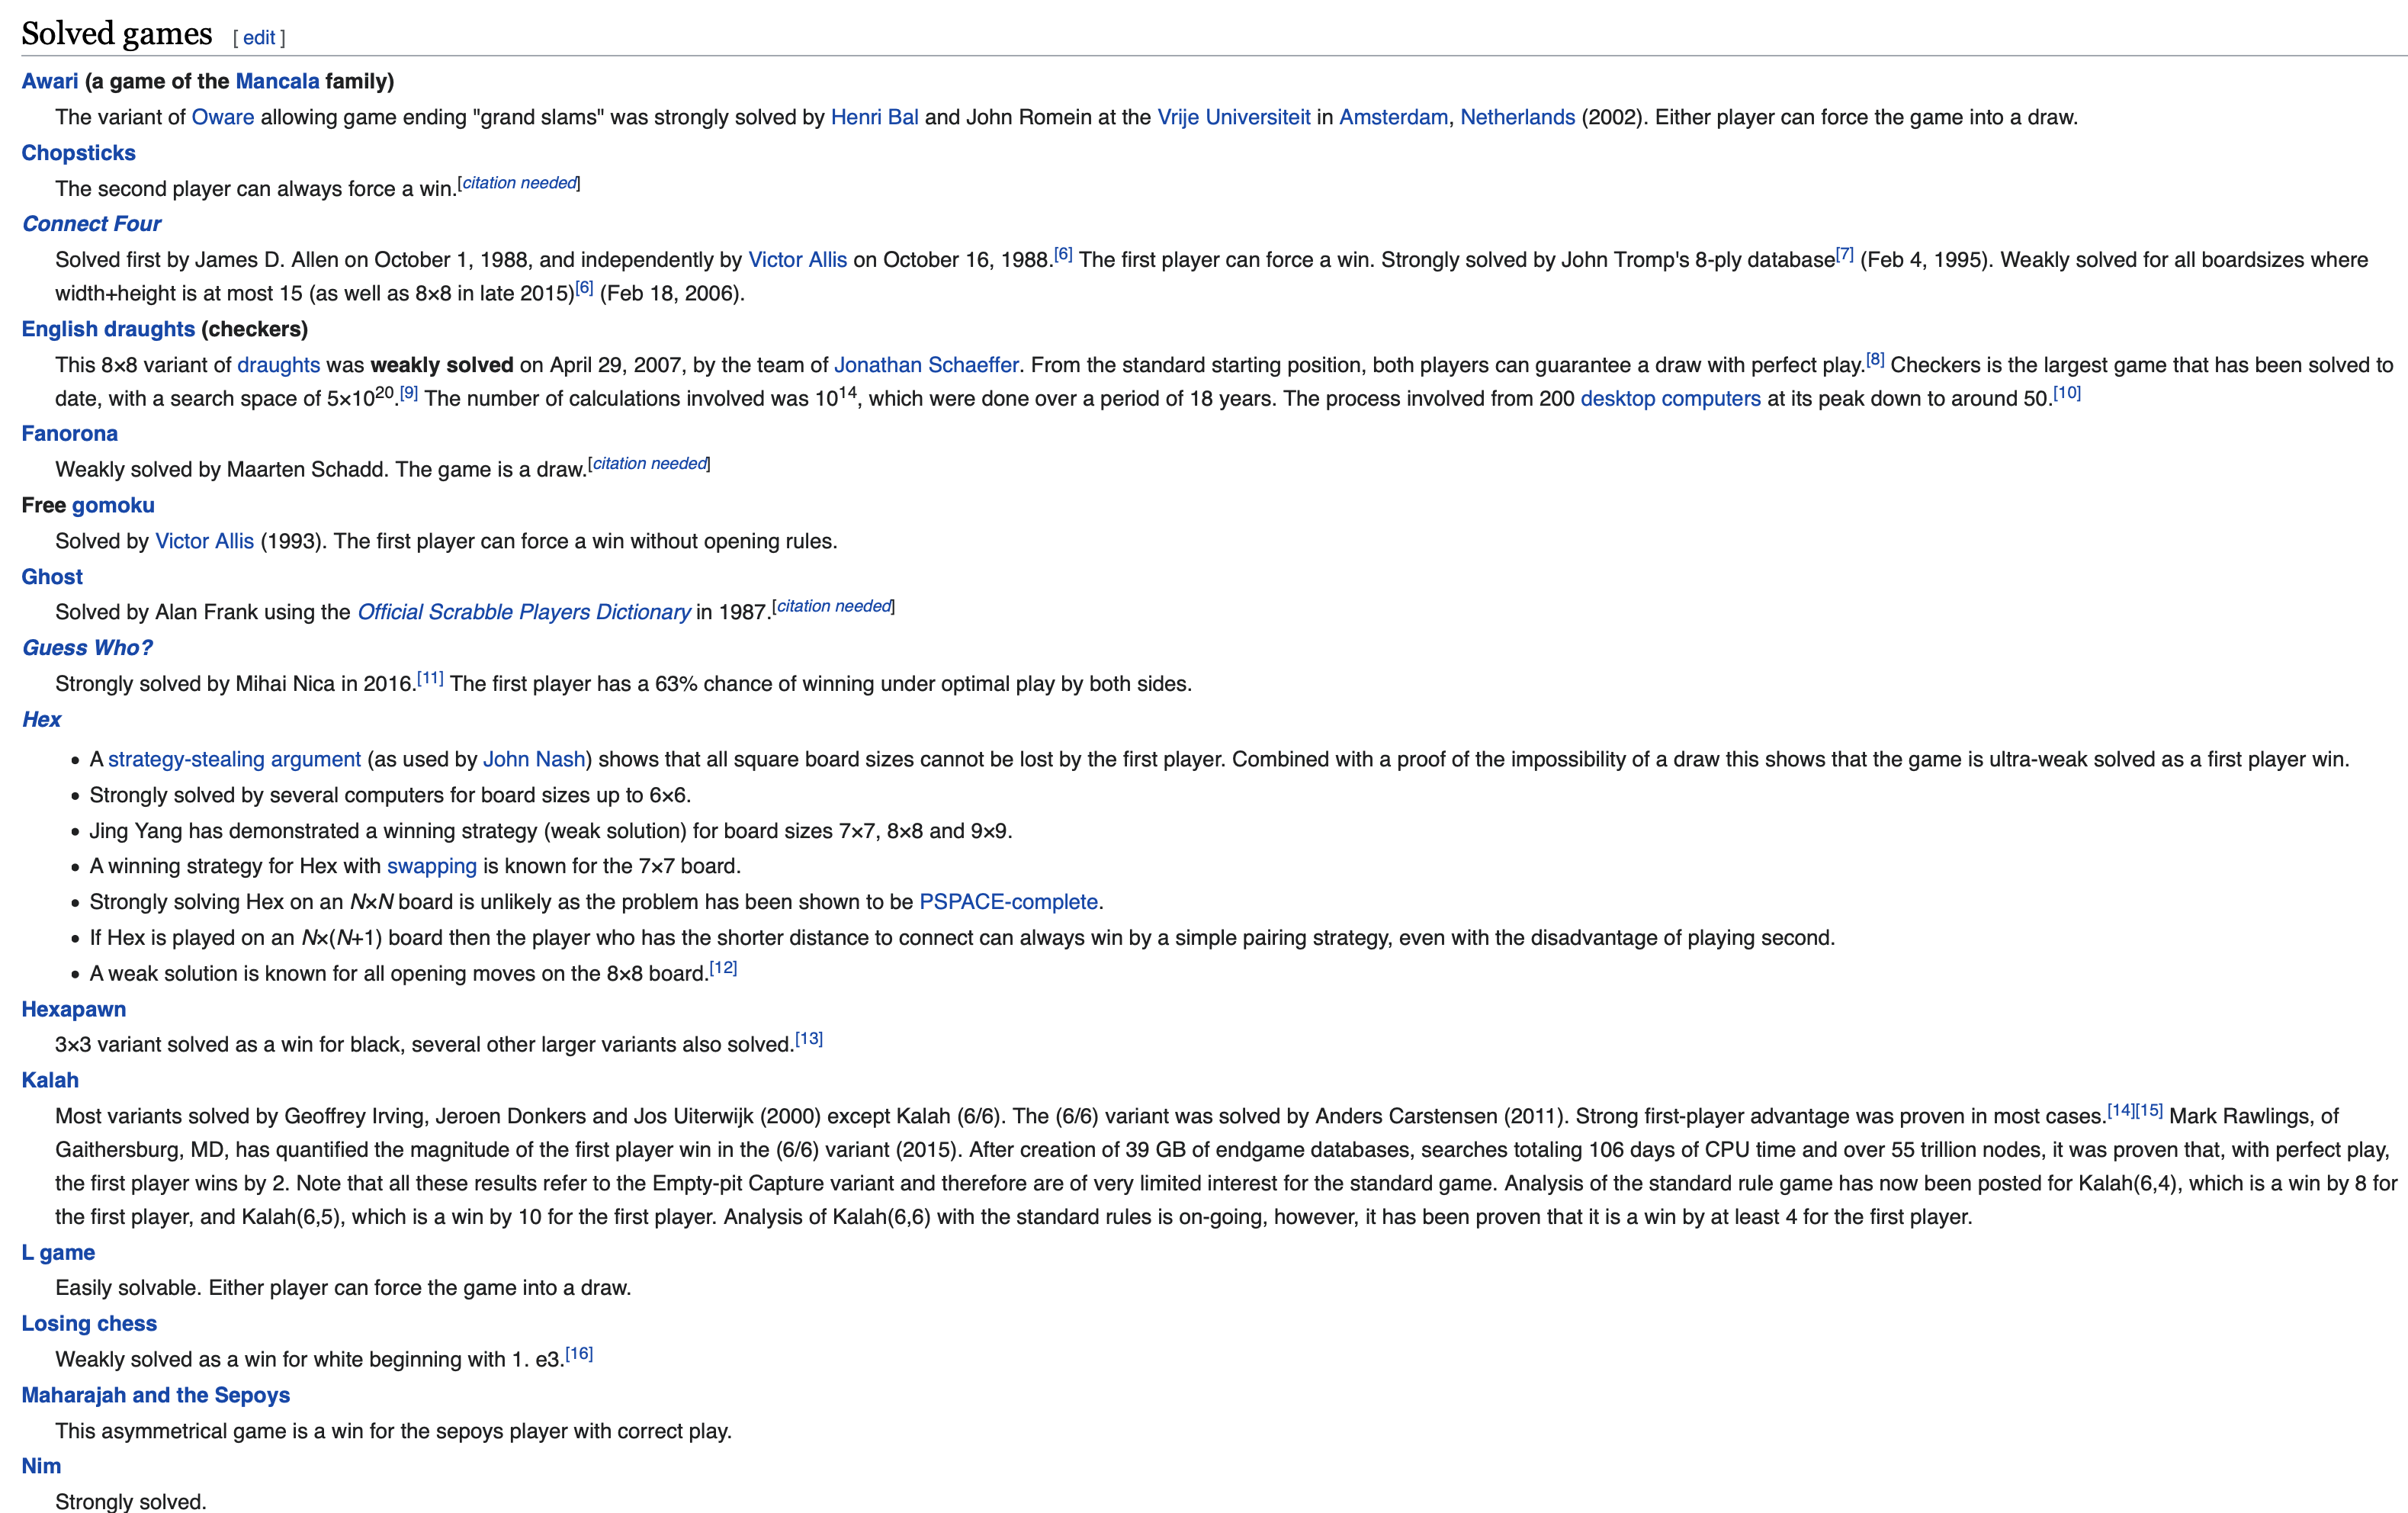
\includegraphics{images/solved.png}
\caption{Wikipedia page on solved games}
\end{figure}
\end{frame}

\begin{frame}{For Next Week}
\protect\hypertarget{for-next-week}{}
We will start chapter 4, on games involving hidden information.
\end{frame}

\end{document}
